\chapter{Bateries}
\label{chap:Bateries}

Avui en dia ens trobem rodejats de bateries: en els telèfons mòbils, en els portàtils, en els automòbils, etc. Hi ha de molts tipus: d'àcid-plom, de níquel i hidrur metàl·lic, de liti... En un futur seran potser l'element més important per a la tecnologia, ja que es convertiran en la font d'energia més emprada per a qualsevol aparell sense fil. 

Per a fer un gestor de bateries, és essencial conèixer el camp de les bateries, de tots els conceptes que cal tenir en compte, tant avantatges com desavantatges i així poder valorar d'una forma més crítica per a la realització d'un prototip, escollir primerament quines serien les bateries que es farien servir, per tal de poder fer un BMS més adaptat a les necessitats d'aquesta. 

\section{Concepte de bateria}

Una bateria és un dispositiu que permet produir electrons a partir d’una reacció química, el que es coneix com reacció electroquímica. Si fem una ullada a qualsevol bateria podem observar com aquesta posseeix dos terminals o bornes. Un d’ells sol estar marcat amb un signe positiu “+” mentre que l’altre posseeix un signe negatiu “-”. Al cablejar aquests dos terminals, els electrons flueixen, tan ràpid com poden, des del terminal negatiu cap al terminal positiu. Normalment es sòl col·locar algun tipus de càrrega en aquesta connexió, com una llum o un motor.

A l’interior de la bateria, una reacció química produeix aquests electrons a una tassa determinada (resistència interna). Per a que la reacció tingui lloc, els electrons han de poder desplaçar-se des del pol negatiu al positiu. Aquesta és la raó per la qual podem teòricament deixar una bateria desconnectada i no perdre aquesta energia. Mentre que si deixem el circuit connectat, el flux d’electrons farà que la bateria es descarregui.

Les bateries es componen d’una o varies cel·les. De fet el terme bateria fa al·lusió a que les cel·les es col·loquen una darrera de l’altre en sèrie per augmentar la capacitat i la tensió de l’acumulador elèctric. Existeix una certa similitud amb el terme pila que es va començar a fer servir perquè les cel·les formen una pila ja que es col·loquen unes damunt de les altres. Però que es una cel·la? Doncs és una espècie de caixa tancada on en el seu interior hi ha dos elèctrodes submergits en un electròlit. Els elèctrodes a la vegada es comuniquen amb l’exterior mitjançant bornes que és on la bateria es connecta al sistema elèctric.

Dintre de les cel·les, entre cada un dels elèctrodes i electròlit, es produeixen unes reaccions químiques reversibles que són las que cedeixen o absorbei- \newline xen electrons. Això genera una tensió elèctrica entre els elèctrodes i per tant entre les dues bornes de la cel·la.                    

\section{Funcionament i usos}
Els processos químics que s'efectuen dins una bateria es coneixen com reaccions redox o de reducció-oxidació. Així dit d'una forma col·loquial en la reducció, els reactius es combinen per a formar altres substàncies químiques més reduïdes i durant aquest procés absorbeixen electrons. \newline L’oxidació és el procés invers. Les substàncies reduïdes es combinen per a formar altres compostos més oxidants i durant el procés s’alliberen \newline càrregues negatives(electrons). Quan la bateria s’està descarregant en \newline l’elèctrode negatiu es produeix una reacció d’oxidació i en el positiu de reducció. Quan la bateria està carregant succeeix l’efecte contrari, l’oxidació es produeix en l'elèctrode positiu i la reducció en el negatiu.

Aquestes reaccions redox no es poden donar de forma indefinida. Després de centenars o milers de cicles de càrrega-descàrrega, el material dels elèctrodes es va debilitant i espatllant de mica a mica a mida que es fan servir fins a espatllar-se completament. Aquesta degradació dels elèctrodes depèn del tipus de tecnologia i de les condicions d’ús: temperatura de funcionament, profunditat de descàrrega...

Actualment, la investigació de millors bateries es centra en la tecnologia d'ions de liti ja que és l’element químic que més tensió genera al produir-se la reacció redox; 3.7V. On s’està treballant per millorar la capacitat de les actuals bateries és en els elèctrodes. Quan major sigui la superfície de contacte dels elèctrodes amb l'electròlit, les reaccions químiques es podran produir en major volum i per tant augmentar la seva capacitat.                 

\section{Mètodes de càrrega de bateries}
L'objectiu d'un carregador és carregar la bateria. Però hi ha moltes altres característiques que poden millorar el funcionament d'un carregador i concedir protecció a la bateria que s'estigui carregant. Aquestes característiques integrades són les que protegeixen la bateria d'un mal funcionament.

Els carregadors de bateries ofereixen característiques o algorismes de \newline càrrega especials els quals tenen com a objectiu millorar el funcionament d'una bateria, reduint el temps de càrrega i augmentant la seva vida útil.

Els conceptes que s'han de tindre en compte a l'hora de dissenyar un carregador de bateria o el algorisme que el controli són:

\begin{itemize}
    \item L'adaptació del voltatge i la intensitat en funció de la temperatura redueix l'evaporació de l'electròlit i els danys en els elèctrodes.
    \item Un alt corrent acabarà reduint la vida útil de la bateria.
    \item La càrrega a polsos pot ajudar a una càrrega complerta.
    \item Una correcta limitació del voltatge redueix l'evaporació de l'electròlit prevenint l'efecte \textit{dry-out}\footnote{Assecament de l'electròlit d'una bateria}.
\end{itemize}

Tradicionalment els carregadors de bateries més simples no regulaven bé els límits de tensió i corrent, únicament es dedicaven a injectar-la. Amb els avenços del sector s'han desenvolupat carregadors de major qualitat capaços de reduir els temps de càrrega, de millorar la protecció contra sobre voltatges i augmentar la vida útil. Tots aquests motius fan que sigui molt més viable treballar amb bateries a nivell econòmic i de seguretat. S'han desenvolupat diferents models els quals seran exposats de forma teòrica a continuació:

\subsubsection{Càrrega a corrent i tensió constants}
És un mètode simple de càrrega que dóna bons resultats sempre i quan els límits de corrent i tensió estiguin ben definits. La càrrega de la bateria comença sent a corrent constant fins que arriba a una determinada tensió en els pols de la bateria. A partir d'aquest moment la càrrega continua però ara a tensió constant i variant la intensitat la qual va reduint-se fins a arribar a un valor en el qual es considera que la bateria està totalment carregada. També es pot controlar si la bateria està completament carregada en funció del temps de càrrega, encara que aquest mètode no és el més aconsellable. 

\subsubsection{Càrrega per goteig}
Aquest mètode és molt semblant a l'anterior, amb la diferència de que aquest permet carregar la bateria fins al 100\% de la seva capacitat. És un mètode efectiu però lent. Aquest tipus de càrrega sol estar associat a bateries d'àcid-plom les quals tenen un corrent baix de gasificació. La idea d'aquest mètode consisteix en subministrar en el procés final de càrrega un corrent molt petit que a condicions de temperatura i tensió pot arribar a ser inferior a una trentena part de la intensitat nominal de la bateria. Aquest mètode de càrrega és també conegut com càrrega de manteniment i s'utilitza per a compensar l'auto-descàrrega de les bateries. 

\subsubsection{Càrrega mitjançant polsos}
Aquest mètode de càrrega consisteix en enviar corrent a la bateria durant períodes molt curts de diversos mil·lisegons en comptes d'estar permanentment amb tensió de càrrega. La duració del pols és la que determina el nivell final de corrent de càrrega subministrada. L'utilització d'un carregador de bateries per polsos aconsegueix mantenir la joventut de la bateria i fer-la viure molt més temps.

\section{Tipus de bateries}
Depenent del material amb el qual estiguin construïts els elèctrodes i de les substancies que formen l’electròlit existeixen diferents tipus de bateries. 

\subsection{Bateries d'un sol ús o recarregables}
Abans de parlar dels tipus de bateries en funció del seu material és important separar els dos grans grups del món de les bateries. Aquests dos grans grups són les bateries recarregables i les d'un sol ús, també conegudes com primàries i secundàries. Les bateries o acumuladors d'un sol ús, com el seu nom indica són d’un únic ús, després es tornen inservibles ja que la reacció química interior s’ha esgotat. Les més comunes d’aquest tipus serien les de zinc carboni o les alcalines, les primeres de menor rendiment que les segones. Les utilitzem en tot tipus d’objectes com comandaments a distància, joguines o llums portàtils... 
\smallskip \newline
Les bateries recarregables ofereixen l’avantatge de tornar a ser carregades per una nova utilització quan han estat descarregades. Les més convencionals són les d'àcid-plom, o conegudes també com bateries humides. Han sigut les utilitzades fins ara en cotxes o motos, per exemple. Les recarregables de major rendiment fins ara han estat d’ions de liti; molt més petites i lleugeres, amb un rendiment superior i una càrrega més ràpida. Aquestes són les utilitzades en dispositius mòbils portàtils, com tauletes o telèfons intel·ligents i en vehicles on es busqui aconseguir un alt rendiment.

\subsection{Bateries o piles alcalines}
Aquests acumuladors són habitualment d'un sol ús i fan servir hidròxid de potassi com el seu electròlit, així com una reacció química entre el zinc i el diòxid de magnesi per generar el corrent elèctric. Les piles alcalines destaquen per un corrent de gran estabilitat, emprades en la majoria de joguines per nens, les llanternes convencionals o els comandaments a distància.

Les piles alcalines han avançat per eliminar el contaminant mercuri que es produïa en el seu interior, de totes maneres, sempre s’han de llençar en punts de recollida de reciclatge, ja que segueixen sent altament contaminants per al medi ambient.

S’han de prendre precaucions amb les piles en desús, en especial amb els nens, ja que pot generar fugues d’hidròxid de potassi, que és altament contaminant i pot generar irritacions a la pell, les vies respiratòries o als ulls. És sempre aconsellable no barrejar piles de diferents tipus, substituir totes les piles quan una s’esgota i guardar-les en un lloc sec quan no fem servir el dispositiu.

\begin{figure}[H]
	\centering
    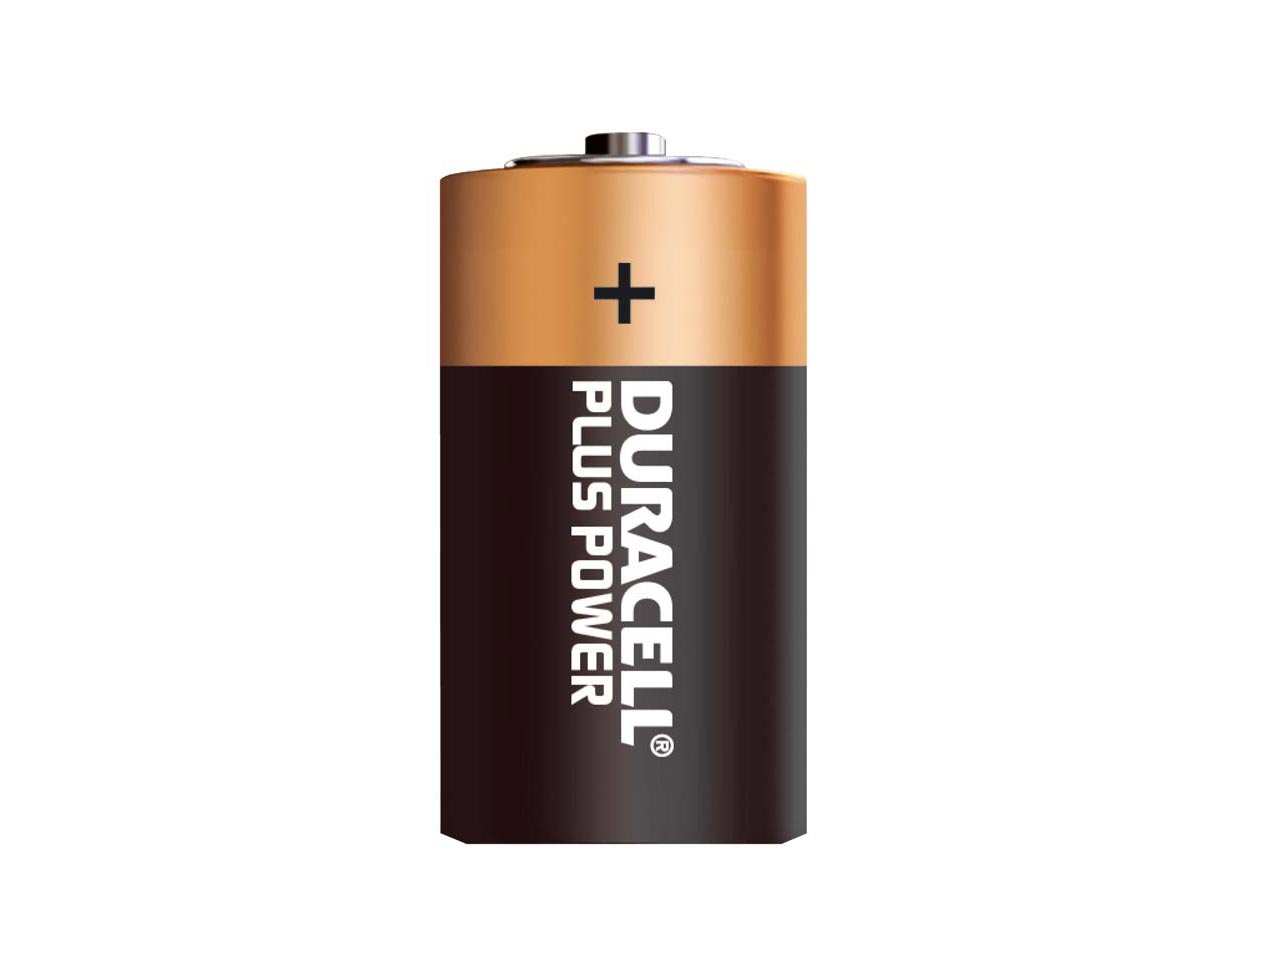
\includegraphics[width=6cm, height=6cm] {Bateries/pilaalcalina.jpg}
    \caption{Bateria o pila alcalina.}
\end{figure}

\subsection{Bateries d'àcid-plom}
Són els acumuladors més comuns fins ara en el món de l’automoció. Aquestes bateries estan formades per dos elèctrodes de plom. Durant el procés de càrrega el sulfat de plom de l’interior perd electrons i es redueix així en plom metall en el seu pol negatiu, mentre que en el pol positiu es forma l'òxid de plom. De la mateixa manera, durant el procés de descàrrega s’inverteix el procés i serà el moment en el que l’òxid de plom format en el pol positiu es transformi un altre cop en sulfat de plom, així com el plom elemental del pol negatiu s’oxidarà per convertir-se igualment en sulfat de plom. Aquest procés genera l’intercanvi d’electrons que aprofitarem per generar energia elèctrica mitjançant un circuit elèctric.

El principal avantatge de les bateries d’àcid-plom és el seu cost, així com una simple fabricació en sèrie. Per contra, són bateries que no es poden sotmetre a sobrecàrregues o descàrregues intenses, són extremadament contaminats, no es caracteritzen per una densitat d’energia massa alta i són molt pesades.

Hem de saber que els acumuladors d’àcid-plom no duren tota la vida, aquestes bateries formen cristalls i serà aleshores quan els processos de carrega-descarrega deixaran d’actuar correctament. Quan això succeeixi no tindrem un altre remei que canviar la bateria, això es coneix com una bateria sulfatada.
\bigskip \bigskip
\begin{figure}[H]
	\centering
    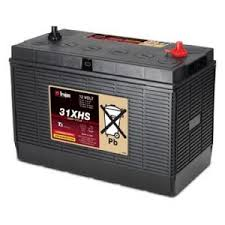
\includegraphics[width=6cm, height=6cm] {Bateries/acidplom.jpg}
    \caption{Bateria d'àcid-plom.}
\end{figure}

\subsection{Bateries de niquel ferro (NI-FE)}
Uns acumuladors formats per uns tubs fins enrotllats per làmines d’acer niquelat formen aquestes bateries. En l’interior dels tubs s’utilitza hidròxid de níquel i com electròlit una barreja de potassa càustica en aigua destil·lada. Aquests acumuladors poden carregar i descarregar perfectament sense efecte memòria ja que formen cristalls de ferro que conserven els elèctrodes en els processos. 

Els acumuladors de níquel ferro són fàcils de fabricar i a un preu baix. A més a més són molt menys contaminants que la resta d’acumuladors, se'ls hi estima una vida útil de més de 80 anys i poden funcionar en qualsevol temperatura damunt l'escorça de la terra. El seu principal inconvenient és un rendiment de només el 65\%. Actualment encara podem trobar algunes funcionant, per emmagatzemar energia generada per plaques solars o turbines eòliques. Per les seves similituds, es diu que les bateries de grafè han ressuscitat aquest tipus de bateries de níquel ferro, encara que això sí, millorant l’inconvenient del rendiment.
\bigskip
\begin{figure}[H]
	\centering
    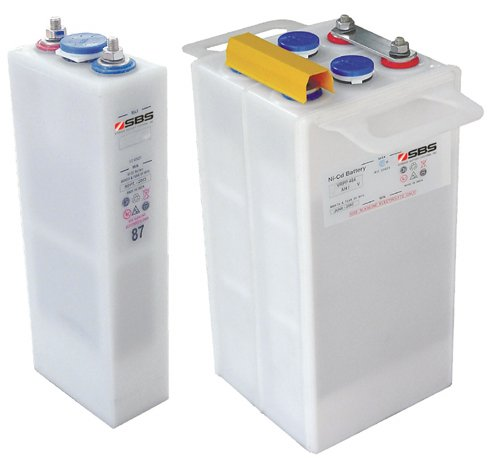
\includegraphics[width=7cm, height=7cm] {Bateries/niquelferro.jpg}
    \caption{Bateria de níquel-ferro}
\end{figure}
\newpage

\subsection{Bateries de níquel-hidrur (Ni-MH)}
Acumuladors que empren un ànode d’hidròxid de níquel i un càtode que està format per una aliatge d’hidrur metàl·lic. Uns acumuladors en els que no preocupen tant la seva càrrega per l’efecte memòria ja que l’aguanten millor que els anteriors. Per contra, no poden ser utilitzades a baixes temperatures ja que perden molt rendiment.

Aquesta classe d’acumuladors de níquel-hidrur són perfectament recarregables i han estat les pioneres en la utilització de vehicles elèctrics. \newline També en l’electrònica de gran consum en forma de pila recarregable, que requereix d'un carregador específic.
\begin{figure}[H]
	\centering
    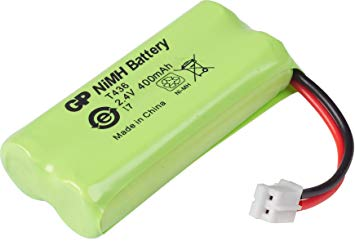
\includegraphics[width=6cm, height=6cm] {Bateries/niquelhidrur.jpg}
    \caption{Bateria de níquel-hidrur.}
\end{figure}

\subsection{Bateries de liti}
Els acumuladors de liti són coneguts actualment com els de major rendiment. La principal competència per a les noves bateries de grafè. Són les utilitzades en l'electrònica de gran consum com tauletes i mòbils intel·ligents, per les seves petites dimensions, reduint el seu pes i donant un excel·lent rendiment fins ara en comparació amb la resta de bateries del mercat.

\subsubsection{Bateries d'ions de liti (Li-Ion)}
Els acumuladors d'ions de liti s’han convertit en els més utilitzats per a dispositius electrònics. Gràcies a la seva sal de liti emprada com electròlit genera la reacció química per fer corrent elèctric. Les bateries d'ions de liti destaquen per la seva alta densitat energètica, acumuladors petits i lleugers amb elevada unitat de càrrega, i per un mínim efecte memòria, és a dir, permeten càrregues i descàrregues sense veure afectat el rendiment de l’acumulador. De totes maneres, en aquesta classe de bateries no tot són avantatges. La seva vida útil es considera mitja, no s’estima que aguantin més de tres anys aproximadament, i la seva duració en les principals aplicacions d'electrònica no és superior a un dia per l’habitual. 
\begin{figure}[H]
	\centering
    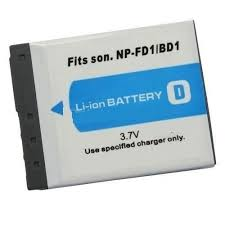
\includegraphics[width=5cm, height=5cm] {Bateries/Li-ion.jpg}
    \caption{Bateria d'ions de liti.}
\end{figure}

\subsubsection{Bateries de polímer d'ions de liti (LiPo)}
Els acumuladors de polímer de liti són una variació de les anteriors. Amb una densitat energètica superior i millores en la tassa de descàrrega. Tot i ser una classe de bateries que milloren les d'ions de liti el seu principal inconvenient és que queden pràcticament inútils si es descarreguen per sota del seu mínim de 3V.
\begin{figure}[H]
	\centering
    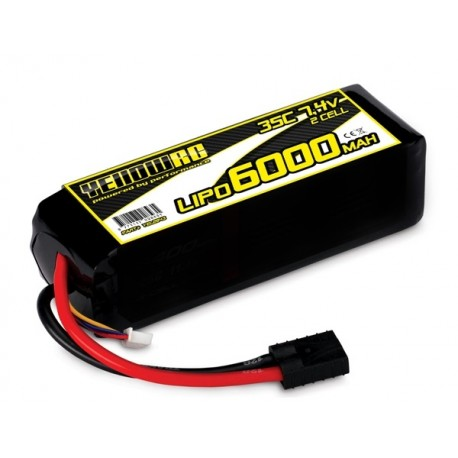
\includegraphics[width=6cm, height=7cm] {Bateries/lipo.jpg}
    \caption{Bateria de polímer d'ions de liti.}
\end{figure}

\subsection{Bateries de grafè}
Aquestes bateries encara estan en desenvolupament. No s’ha acabat de trobar encara un equilibri que pugui estabilitzar el pros i els contres \newline d’aquest tipus de bateries. Els polímers de grafè són un nano material format per carboni pur amb àtoms disposats en patró hexagonal. En el fons es tracta d’un material molt similar al grafit, però amb major duresa, flexibilitat i elasticitat. No obstant, el punt més interessant d’aquest nano-material transparent és la seva altíssima conductivitat elèctrica, a més a més de la seva capacitat per generar electricitat al ser assolits per la llum. 
En termes pràctics, les bateries de grafè tenen una velocitat de càrrega molt més ràpida i una densitat d’energia moltíssim més elevada que el que mai podran oferir les bateries d’ions de liti. També un altre punt a tenir en compte és que són molt menys pesades que les bateries habituals. Això porta lloc a un gran interès sobre aquestes bateries en el món de l’automoció, ja que es pot arribar a reduir el pes de la bateria fins a un 75\% a més a més de donar totes les característiques esmentades anteriorment.
\begin{figure}[H]
	\centering
    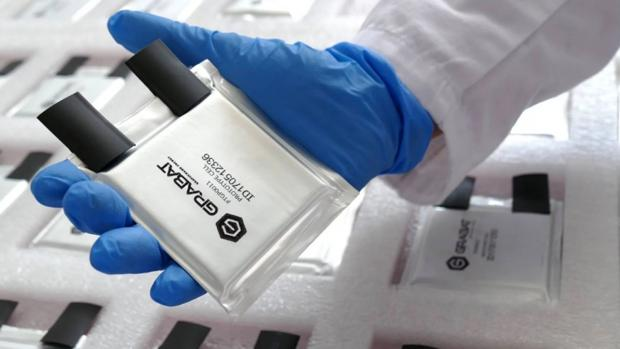
\includegraphics[width=9cm, height=7cm] {Bateries/grafeno.jpg}
    \caption{Bateria de grafè.}
\end{figure}                                    

\section{Bateries de liti com a font d'energia per al nostre vehicle elèctric}
En primer lloc el que cal saber per entendre millor aquest tipus de bateries és tindre un petit coneixement de les característiques que permet el liti. El liti és un metall alcalí, inflamable, blanc platejat, dúctil i molt poc pesat que es caracteritza per corroir-se amb rapidesa quan entra en contacte amb l’aire. No existeix en estat lliure en la naturalesa encara que si està present en compostos com en l'escorça terrestre. La presència del liti en la naturalesa és molt comuna ja que es troba en 65 parts per milió de l'escorça terrestre. A més a més el liti no es pot submergir sota l’aigua perquè podria cremar i el contacte amb la pell podria ocasionar lesions, pel que és indispensable que el fabricant de les bateries de liti compti amb materials i mètodes de fabricació que compleixin la normativa i exigències vigents. Encara que nombroses investigacions afirmin que el liti té propietats molt interessants que encara no s’han estudiat en profunditat, actualment l’ús principal del liti és per a les bateries de liti, oferint excel·lents propietats en comparació amb altres tipus de bateries molt comunes en el mercat.

Les bateries de liti, es caracteritzen per carregar-se més ràpid, durar més, comptar amb una major vida útil i oferir més densitat energètica, pel que en menys espai es pot obtenir una major autonomia i treure-li més partit a les bateries de liti.

\begin{figure}[H]
	\centering
    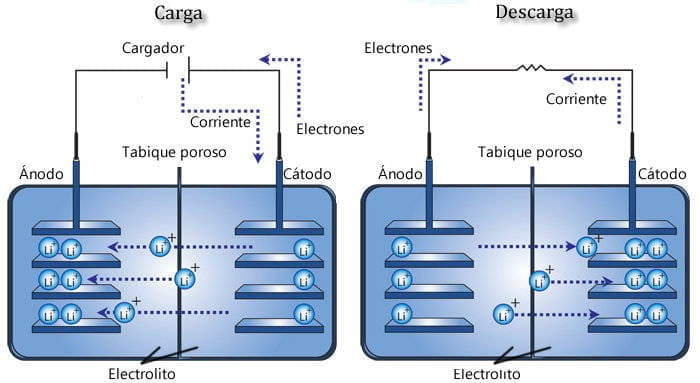
\includegraphics[width=\textwidth, height=7cm] {Bateries/cargadescargalitio.jpg}
    \caption{Funcionament d'una bateria de liti}
\end{figure}

Existeixen tres tipus de bateries de liti:
\begin{itemize}
    \item Bateries d’òxid de cobalt/liti: Tenen el benefici de l’alta densitat \newline d’energia, que encara que a vegades pugui comportar problemes de seguretat, solen tractar-se de bateries de gran durabilitat.
    \item Bateries de liti/òxid de magnesi: Es tracta de la bateria més emprada pel seu alt nivell de seguretat, però el seu rendiment no sempre és eficient quan s’experimenten altes temperatures.
    \item Bateries de liti/fosfat de ferro: Es tracta de la bateria amb les majors característiques de seguretat amb una llarga vida útil, de més de 2000 cicles. 
\end{itemize}

\subsection{Bateries d'ions de liti}
Les bateries d'ions de liti són un dispositiu dissenyat per a \newline l'emmagatzemament d’energia elèctrica que empra com electròlit una sal de liti que aconsegueix els ions necessaris per a la reacció electroquímica reversible que té lloc entre el càtode i l'ànode.

Les propietats de las bateries de Li-Ion, com la lleugeresa dels seus component, la seva elevada capacitat energètica i resistència a la descarrega, juntament amb el poc efecte memòria que sofreixen o la seva capacitat per a funcionar a un elevat nombre de cicles de regeneració, ha permès dissenyar acumuladors lleugers, de petita mida i variades formes, amb un alt rendiment, especialment adaptats a les aplicacions de la indústria electrònica de gran consum. Des de la primera comercialització d’un acumulador basat en la tecnologia Li-Ion a principis dels anys 90, el seu ús s’ha popularitzat en aparells com telèfons mòbils, agendes electròniques, ordinadors portàtils i lectors de música.

No obstant, la seva ràpida degradació i sensibilitat a les altes temperatures, que pot resultar en la destrucció per inflamació o inclús explosió, requereixen, en la seva configuració com a producte de consum, la inclusió de dispositius addicionals de seguretat, resultant en un cost superior que ha limitat l’extensió del seu ús a altres aplicacions.

En el context del creixent encariment de combustibles derivats del petroli, la industria de l'automòbil ha anunciat el seu desenvolupament, proliferació i comercialització de vehicles amb motors elèctrics basats en la tecnologia de les bateries d’ions de liti, amb els que es pugui disminuir la dependència energètica d’aquestes fonts a la vegada que es manté la baixa emissió de gasos contaminants.

\subsection{Bateria de polímer de liti (LiPo)}

Les bateries de polímer d'ions de liti són piles recarregables, compostes generalment de vàries cel·les secundàries idèntiques en paral·lel per augmentar la capacitat del corrent de descàrrega, i estan sovint disponibles en sèries de paquets per augmentar el voltatge total disponible.

Les bateries LiPo funcionen seguint el mateix principi que les bateries d'ions de liti, l’intercanvi d’electrons entre el material de l'elèctrode \newline negatiu i el material de l'elèctrode positiu mitjançant un conductor. Per evitar que els elèctrodes es toquin directament, es col·loca entre ells un material amb porus microscòpics, que permeten tan sols als ions de liti (i no a les partícules dels elèctrodes) migrar d’un elèctrode a l'altre.

Les bateries LiPo estan classificades pel numero de cel·les “S” pel qual estan formades. Així una bateria 4S estaria composta per 4 sub-bateries connectades en sèrie. A més a més la capacitat d’aquestes bateries queda indicada en “mAh”. A major nombre de mil·liamperes (mAh) més capacitat de càrrega. Quan parlem d’una bateria amb una capacitat de 2200 mAh estem dient que aquesta bateria és capaç de descarregar a 2,2 A en una hora.

\subsection{Avantatges i desavantatges de les bateries LiPo}

Els principals avantatges i desavantatges que tenen aquestes bateries són els següents:
\begin{itemize}
    \item No presenta sulfatació.
    \item Alta densitat de càrrega.
    \item No existeix la necessitat d'una càrrega prolongada quan són noves.
    \item Índex d'auto-descàrrega baix.
    \item Són bateries que generen un menor impacte en el medi ambient.
    \item Varietat de models disponibles tant en càrrega com en mida, un fet molt important que li dona versatilitat.
    \item No requereixen de tant manteniment com altres bateries, no necessiten descàrregues periòdiques ja que no presenten efecte memòria.
\end{itemize}

Però no tot són avantatges. També presenten una sèrie de desavantatges a tenir molt en compte:
\begin{itemize}
    \item Envelliment: Les bateries d'ions de liti estan exposades a envelliment per diversos motius. Un excés de temperatura, un elevat nombre de càrregues i descàrregues que provoca una degradació, també la provoca (i en això és on es diferencia d'altres tipus de bateries) el deteriorament durant el temps que estan emmagatzemades amb càrrega. 
    \item Requereixen protecció: Les cel·les d'ions de liti no són tan robustes com altres tecnologies recarregables. Han de tenir un sistema de protecció davant de sobrecàrregues i descàrregues profundes, temperatura...
    \item Cost: Les bateries LiPo tenen un cost de fabricació més alt que altres bateries.
    \item Rapid disassembly: Aquest és un dels problemes en els que més es treballa per evitar. Es pot donar per la presència de partícules metàl·liques microscòpiques que arriben a curtcircuitar la cel·la, però aquesta causa és cada cop més rara ja que els fabricants de bateries s'enfoquen en l'eliminació d'aquestes partícules, encara que l'eliminació total d'aquestes és impossible. Però el verdader problema està en que els curtcircuits es provoquin dins la cel·la, allà les proteccions externes són ineficaces per parar la reacció que es produeix. Si degut a un defecte en la bateria o a un mal ús d'aquesta la bateria s'escalfa en excés, aquesta temperatura pot afectar a la integritat de la capa d'aïllament d'una de les cel·les. Si aquesta capa falla es produeix un curtcircuit en que les temperatures poden arribar als 500ºC i la cel·la pot incendiar-se o explotar. Això a la vegada pot afectar a les cel·les properes i pot originar una reacció en cadena. 
\end{itemize}

\subsection{Riscs en l'ús de bateries LiPo}

El funcionament i la qualitat d'una bateria LiPo ve determinat pel \newline voltatge donat per la cel·la i la temperatura d'aquesta. Aquests són els factors més importants a tenir present sobre una bateria LiPo. 

\subsubsection{Riscs en la sobrecàrrega}
Si el voltatge de càrrega s'incrementa per sobre del seu màxim aconsellable de 4,2V provoca que circuli un corrent excessiu, el que deriva als següents problemes:
\begin{itemize}
    \item Sobreescalfament: Un excés de corrent en la càrrega incrementa \newline l'escalfament de la cel·la. 
    \item Formació de plaques de liti: Quan el corrent de càrrega resulta excessiu , els ions de liti no s'acomoden suficientment ràpid entre els estrats d'intercalació de l'ànode, sinó que s'acumulen en la superfície de l'ànode formant una placa de liti metàl·lic. Aquesta formació de plaques es tradueix en que després en la descàrrega hi haurà una quantitat menor d'ions de liti lliures suposant una pèrdua de capacitat de la bateria. 
\end{itemize}

\subsubsection{Riscs en la sobre descàrrega}
De la mateixa manera que sotmetre a la cel·la a un voltatge de càrrega excessiu causa problemes el descarregar-la en excés genera un molt important que és la descomposició dels materials dels elèctrodes.
\begin{itemize}
    \item Càtode: Mantenir les cel·les a voltatges inferiors de 2 volts de manera prolongada provoca la descomposició gradual del càtode. Durant aquesta descomposició s'allibera oxigen de l'òxid de liti tot provocant un augment de la pressió dins de la cel·la. Es pot arribar a manifestar d'una forma violenta si no disposen d'una sortida més controlada.   
   \item Ànode: El col·lector de corrent de l'ànode de coure es dissol en \newline l'electròlit. Aquest provoca que augmenti l'auto descàrrega de la bateria i que quan s'intenti recarregar la cel·la, en el moment que el seu voltatge augmenti en dos volts, els ions de coure que s'han dissolt en l'electròlit es precipitaran com coure metàl·lic i no necessàriament es dipositaran en el dipòsit de coure de l'ànode. Això és un comportament de risc que pot causar en última instància un curtcircuit entre elèctrodes.

\end{itemize}

\subsubsection{Riscs a baixes temperatures de funcionament}
L'índex de reaccions químiques està relacionat amb la temperatura. \newline La reducció de la temperatura de funcionament d'una cel·la implica reduir el nombre de reaccions químiques que es produeixen dins d'aquesta. Això es tradueix en una reducció del corrent que pot suportar la cel·la durant la càrrega i la descàrrega. Implica una pèrdua de potència útil de la cel·la i un augment del dany generat a aquesta durant la càrrega. Si es carrega la cel·la amb un corrent superior a l'admissible els ions de liti en comptes d'inserir-se entre els estrats es dedicaran a formar plaques de liti.


\subsubsection{Riscs a altes temperatures de funcionament}
Operar a temperatures excessives produeix una sèrie de problemes, la majoria relacionats amb la destrucció de la cel·la. Una temperatura elevada provoca un augment del nombre de reaccions químiques que es produeixen en la cel·la i fa que el corrent de la cel·la augmenti. Això que en principi sembla bo no ho és ja que un augment en el corrent ve de la mà amb un augment de la potència dissipada en la resistència interna de la cel·la, potència que es dissipa en escalfor i fa que encara augmenti més la temperatura. De no controlar-ho a la cel·la succeiria una fuga tèrmica.

\subsubsection{Fuga tèrmica}
La primera etapa en una fuga tèrmica és la destrucció de la capa SEI\footnote{Solid Electrolyte Interface} en l'ànode degut a un sobreescalfament d'aquesta o a una perforació. El sobreescalfament pot estar produït per un excessiu corrent, una sobrecàrrega de la cel·la o per una temperatura ambient massa elevada. La destrucció d'aquest estrat comença a una temperatura relativament baixa, 80ºC. Un cop que es danya la capa l'electròlit reacciona amb l'ànode de carboni tal i com succeeix durant la formació original de la capa SEI, ara d'una manera més descontrolada. Considerant que és una reacció exotèrmica contribueix a aquest augment de temperatura de la cel·la. 

A mesura que la temperatura de la cel·la creix el calor generat en l'ànode provoca la descomposició dels dissolvents orgànics emprats en l'electròlit alliberant aquests gasos inflamables com el metà. Aquesta descomposició sol començar als 110º, això depèn de la naturalesa de l'electròlit on en alguns casos pot arribar a començar als 70º. El gas generat s'acumula augmentant la pressió dins la cel·la. Encara que la temperatura de la cel·la augmenti per sobre del punt d'inflamació no s'inicia la combustió degut a que no hi ha oxigen. Les cel·les solen estar equipades amb algun mecanisme capaç d'alliberar pressió de la cel·la sense posar a aquesta en risc, evitant així l'explosió. Però una vegada els gasos són alliberats a l'atmosfera i a aquesta temperatura cremen.

Als 135º aproximadament es fon el separador provocant un curtcircuit entre els dos elèctrodes. L'escalfor generat en aquest curtcircuit provoca la descomposició de l'òxid del càtode el que allibera oxigen, tot permetent que els gasos i l'electròlit que queden a l'interior de la cel·la cremin,. Aquesta combustió eleva tant la temperatura i la pressió de la cel·la que aquesta explota. La temperatura a la qual es sol descompondre el càtode és d'aproximadament 200ºC.

\subsection{Seguretats a tenir en compte en les bateries LiPo}

Les bateries LiPo són bastant delicades. Si bé una bateria amb bon ús i bon manteniment pot arribar a realitzar més de 300 cicles de càrrega i descàrrega, una bateria mal cuidada pot no arribar ni als 50 cicles. A més a més, el seu ús incorrecte, en especial les sobrecàrregues, pot produir que les bateries LiPo cremin. Per això, per treballar amb bateries de forma segura i per allargar la vida útil de les mateixes, és important seguir uns certs consells:

\begin{itemize}
    \item Mai deixar desateses les bateries mentre carreguen, poden cremar. \item Carregar-les en un lloc on no hi hagi materials inflamables. 
    \item Necessari carregar-les amb un carregador específic.
    \item Mai s'ha de deixar que els terminals entrin en contacte entre ells, ja que això provocaria un curt-circuit i podria fer que la bateria \newline s'incendiés.
    \item Deixar refredar les bateries a la temperatura ambient després de fer-les servir abans de carregar-les.
    \item Mai carregar les bateries per sobre del voltatge indicat pel fabricant. Hi ha perill que cremin. Tampoc s'han de carregar en llocs molt freds (menys de 5ºC) ni molt calents. La temperatura ideal de funcionament d'una bateria LiPo es troba entre els 30 i 40ºC. Per sota, la bateria no treballa al 100\% i per sobre de 60ºC la bateria ja comença a malmetre's. 
\end{itemize}
La millor forma d'emmagatzemar les bateries durant molt temps és deixant-les a un 40\% de la seva càrrega. Ha de ser un lloc sec i a una temperatura entre 5 i 25ºC.Existeixen fundes especials ignífugues que s'utilitzen per emmagatzemar les bateries de forma segura.

Mai s'ha de fer servir una bateria que es vegi danyada o voluminosa. Si en qualsevol moment s'observa que la bateria LiPo s'infla o derrama líquid, cal desconnectar-la i observar-la durant uns 10 minuts o 20 minuts en un lloc segur. Això podria provocar l'ignició de la bateria degut als components químics que entren en contacte amb l'aire.

\subsection{Característiques de la càrrega de bateries LiPo}
Per seguretat i per prolongar la vida de la bateria hem de tenir en compte com es realitza una càrrega segura d'una bateria d'ions de liti. A continuació es mostrarà el procés de càrrega d'una cel·la d'ions de liti, en una càrrega genèrica no una específica.

Concretament estem parlant de bateries de Li-ion fabricades amb els materials de càtode tradicionals de cobalt, níquel, manganès i alumini de càrrega típicament a 4.2V/cel·la. La tolerància es +/- 50mV/cel·la. 

Un dels principals conceptes que s'han de tenir en compte és que en les bateries de liti els voltatges de tall no tenen una flexibilitat com altres bateries. En augmentar el voltatge també s'augmenta la capacitat, però anar més enllà de l'especificació pot sobrecarregar la bateria. Els circuits de protecció incorporats en el paquet no permeten excedir el voltatge establert.
Voltatges més alts provocarien estrès a la bateria, comportant a una reducció de la seva vida útil. És més preocupant el problema de seguretat que pot comportar aquest excés de tensió.

A continuació es mostrarà una gràfica en la que es poden veure les diferents fases de càrrega de la cel·la.

\begin{figure}[H]
	\centering
    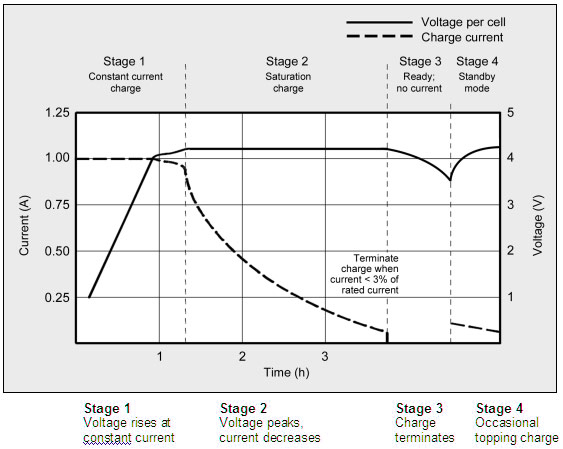
\includegraphics[width=\textwidth, height=8cm] {Bateries/cargabatlipo.jpg}
    \caption{Etapes de càrrega d'una bateria LiPo.}
\end{figure}

A l'etapa 1 es veu com la velocitat de càrrega d'una bateria típica és d'entre 0,5 i 1A. La càrrega complerta es produeix quan la bateria arriba al llindar de voltatge i el corrent cau al tres per cent del corrent nominal. Aquest punt es pot apreciar al final de l'etapa 2 i inici de l'etapa 3. En lloc de càrrega lenta, alguns carregadors apliquen una càrrega màxima quan la tensió cau a 4.05V/cell (etapa 4).

El temps total de càrrega és aproximadament d'unes tres hores en funció del mètode de càrrega. Quan la bateria queda completament carregada la seva temperatura pot augmentar fins a 5ºC. Si s'augmenta el corrent de càrrega la bateria no es carregarà abans, sinó que arribarà abans al pic de tensió. No obstant  l'etapa 2 (saturació) requerirà més temps.

Una bateria de liti no pot absorbir la sobrecàrrega i és precís que quan s'arribi a la càrrega complerta el corrent sigui tallat. Si aquest continua es poden formar plaques de liti metàl·lic que són un factor de perill ja que poden causar curtcircuits. També augmenta l'estrès de la bateria si es manté durant un bon temps el voltatge de pic de 4,2V.

Un cop que la càrrega es termina, el voltatge de la bateria comença a disminuir, el que alleuja l'estrès de tensió. Amb el temps, el voltatge de circuit obert s'assentarà entre 3,6 i 3,9V/cel·la. S'ha de tenir en compte que una bateria de Li-ion que ha rebut una càrrega totalment saturada mantindrà la tensió més alta que una on la seva càrrega ha estat ràpida i sense càrrega de saturació.

La següent gràfica mostra la relació entre tensió, corrent i capacitat que succeeix en la càrrega d'una cel·la.

\begin{figure}[H]
	\centering
    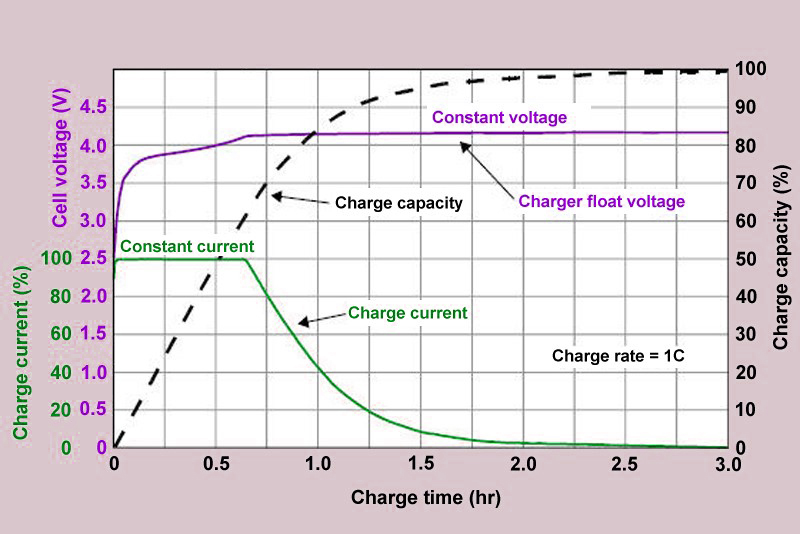
\includegraphics[width=\textwidth, height=7cm] {Bateries/VICgrafica.jpg}
    \caption{Evolució del voltatge, el corrent i la capacitat en la càrrega d'una bateria LiPo.}
\end{figure}

Alguns carregadors apliquen una breu càrrega d'anivellació per compensar la petita auto-descàrrega de la bateria i el consum del circuit de protecció. El carregador pot arrencar quan el voltatge de circuit obert de la cel·la cau a 4.05V i tanca de nou a 4.2V.

Un dispositiu portàtil ha d'estar apagat durant la càrrega. Això permet que la bateria arribi a un voltatge llindar establert sense problemes, i permet acabar la càrrega amb corrent baix. Una càrrega parasitària confon el carregador mitjançant la pulsació de la tensió de la bateria i altera la mesura del corrent en la fase de saturació.

Les bateries d'aquest tipus treballen amb seguretat dins dels límits fixats però es tornen inestables si es sobrecarreguen amb una tensió superior a l'especificada. Es comencen a formar plaques de liti en l'ànode mentre que en el càtode es produeix un material oxidant, perd estabilitat i produeix CO2. Si no s'activa cap mecanisme de seguretat pot desencadenar en una fuga tèrmica. 

\subsection{Característiques de la descàrrega de bateries LiPo}

Les cel·les d'una bateria de liti no han de ser descarregades massa, per norma l'equip hauria d'interrompre la descàrrega quan el voltatge d'una cel·la arribi als 3V. Si el seu voltatge baixa dels 2.7V el circuit de protecció de la bateria posarà la bateria en mode espera i una recàrrega ja no serà possible amb la majoria dels carregadors comercials. No s'han de recarregar cel·les on la tensió hagi caigut per sota dels 1,5V doncs poden haver-se format derivacions de coure en l'interior de l'ànode i poden produir un curtcircuit.

A continuació es mostrarà una gràfica en la que es pot veure la relació del voltatge en funció de la capacitat durant la descàrrega a diferents intensitats.

\begin{figure}[H]
	\centering
    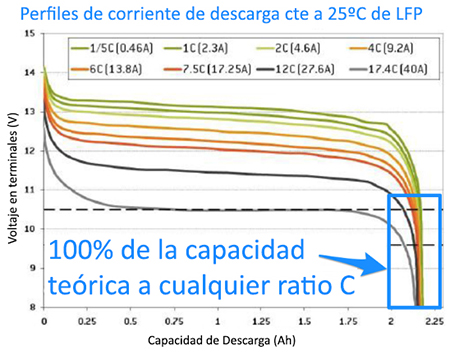
\includegraphics[width=10cm, height=10cm] {Bateries/graficadescargabatlipo.jpg}
    \caption{Descàrrega d'una bateria LiPo a diferents intensitats.}
\end{figure}
